\documentclass[11pt,openany]{article}

\usepackage{mathtools, commath}
% Packages for formatting
\usepackage[margin=1in]{geometry}
\usepackage{fancyhdr}
\usepackage{enumerate}
\usepackage{graphicx}
\usepackage{kotex}
\usepackage{arydshln} % Include this package
\usepackage{bbding}
\usepackage{amsmath}
\usepackage{amsthm}
\usepackage[dvipsnames,table]{xcolor}
\usepackage{amssymb, amsfonts}
\usepackage{wasysym}
\usepackage{footnote}
\usepackage{tablefootnote}
\usepackage{arydshln} % Include this package
% Fonts
\usepackage[T1]{fontenc}
\usepackage[utf8]{inputenc}
\usepackage{newpxtext,newpxmath}
\usepackage{sectsty}

% Define colors
\definecolor{TealBlue1}{HTML}{0077c2}
\definecolor{TealBlue2}{HTML}{00a5e6}
\definecolor{TealBlue3}{HTML}{b3e0ff}
\definecolor{TealBlue4}{HTML}{00293c}
\definecolor{TealBlue5}{HTML}{e6f7ff}

\definecolor{thmcolor}{RGB}{231, 76, 60}
\definecolor{defcolor}{RGB}{52, 152, 219}
\definecolor{lemcolor}{RGB}{155, 89, 182}
\definecolor{corcolor}{RGB}{46, 204, 113}
\definecolor{procolor}{RGB}{241, 196, 15}

\usepackage{color,soul}
\usepackage{soul}
\newcommand{\mathcolorbox}[2]{\colorbox{#1}{$\displaystyle #2$}}
\usepackage{cancel}
\newcommand\crossout[3][black]{\renewcommand\CancelColor{\color{#1}}\cancelto{#2}{#3}}
\newcommand\ncrossout[2][black]{\renewcommand\CancelColor{\color{#1}}\cancel{#2}}

\usepackage{hyperref}
\usepackage{booktabs}

% Chapter formatting
\definecolor{titleTealBlue}{RGB}{0,53,128}
\usepackage{titlesec}
\titleformat{\section}
{\normalfont\sffamily\Large\bfseries\color{titleTealBlue!100!gray}}{\thesection}{1em}{}
\titleformat{\subsection}
{\normalfont\sffamily\large\bfseries\color{titleTealBlue!50!gray}}{\thesubsection}{1em}{}

%Tcolorbox
\usepackage[most]{tcolorbox}
\usepackage{multirow}
\usepackage{multicol}

\usepackage[linesnumbered,ruled]{algorithm2e}
\usepackage{algpseudocode}
\usepackage{setspace}
\SetKwComment{Comment}{/* }{ */}
\SetKwProg{Fn}{Function}{:}{end}
\SetKw{End}{end}
\SetKw{DownTo}{downto}

% Define a new environment for algorithms without line numbers
\newenvironment{algorithm2}[1][]{
	% Save the current state of the algorithm counter
	\newcounter{tempCounter}
	\setcounter{tempCounter}{\value{algocf}}
	% redefine the algorithm numbering (remove prefix)
	\renewcommand{\thealgocf}{}
	\begin{algorithm}
	}{
	\end{algorithm}
	% Restore the algorithm counter state
	\setcounter{algocf}{\value{tempCounter}}
}

\usepackage{adjustbox}
% Header and footer formatting
\pagestyle{fancy}
\fancyhead{}
\fancyhf{}
\rhead{\textcolor{TealBlue2}{\large\textbf{기대수(기초부터 대학원 수학까지 시리즈) 3기}}}%\rule{3cm}{0.4pt}}
\lhead{\textcolor{TealBlue2}{\large\textbf{수학의 즐거움, Enjoying Math}}}
% Define footer
%\newcommand{\footer}[1]{
%\begin{flushright}
%	\vspace{2em}
%	\includegraphics[width=2.5cm]{school_logo.jpg} \\
%	\vspace{1em}
%	\textcolor{TealBlue2}{\small\textbf{#1}}
%\end{flushright}
%}
%\rfoot{\large Department of Information Security, Cryptogrphy and Mathematics, Kookmin Uni.\includegraphics[height=1.5cm]{school_logo.jpg}}
\fancyfoot{}
\fancyfoot[C]{-\thepage-}

\usepackage{tcolorbox}
\tcbset{colback=white, arc=5pt}

\definecolor{axiomcolor}{HTML}{a88bfa}
\definecolor{defcolor}{RGB}{52, 152, 219}
\definecolor{procolor}{RGB}{241, 196, 15}
\definecolor{thmcolor}{RGB}{231, 76, 60}
\definecolor{lemcolor}{RGB}{155, 89, 182}
\definecolor{corcolor}{RGB}{46, 204, 113}
\definecolor{execolor}{RGB}{90, 128, 127}

% Define a new command for the custom tcolorbox
\newcommand{\axiombox}[2][]{%
	\begin{tcolorbox}[colframe=axiomcolor, title={\color{white}\bfseries #1}]
		#2
	\end{tcolorbox}
}

\newcommand{\defbox}[2][]{%
	\begin{tcolorbox}[colframe=defcolor, title={\color{white}\bfseries #1}]
		#2
	\end{tcolorbox}
}

\newcommand{\lembox}[2][]{%
	\begin{tcolorbox}[colframe=lemcolor, title={\color{white}\bfseries #1}]
		#2
	\end{tcolorbox}
}

\newcommand{\probox}[2][]{%
	\begin{tcolorbox}[colframe=procolor, title={\color{white}\bfseries #1}]
		#2
	\end{tcolorbox}
}

\newcommand{\thmbox}[2][]{%
	\begin{tcolorbox}[colframe=thmcolor, title={\color{white}\bfseries #1}]
		#2
	\end{tcolorbox}
}

\newcommand{\corbox}[2][]{%
	\begin{tcolorbox}[colframe=corcolor, title={\color{white}\bfseries #1}]
		#2
	\end{tcolorbox}
}



\usepackage{amsthm}

% Define custom theorem styles
\newtheoremstyle{dotless} % Name of the style
{3pt} % Space above
{3pt} % Space below
{\itshape} % Body font
{} % Indent amount
{\bfseries} % Theorem head font
{} % Punctuation after theorem head
{2.5mm} % Space after theorem head
{} % Theorem head spec

\newtheoremstyle{definitionstyle} % Name of the style
{3pt} % Space above
{3pt} % Space below
{} % Body font
{} % Indent amount
{\bfseries} % Theorem head font
{.} % Punctuation after theorem head
{2.5mm} % Space after theorem head
{} % Theorem head spec

% Applying custom styles
\theoremstyle{dotless}
\newtheorem{theorem}{Theorem} % Theorem environment with section-wise numbering
\newtheorem{proposition}[theorem]{Proposition} % Theorem environment with section-wise numbering
\newtheorem{lemma}[theorem]{Lemma} % Lemma shares the counter with theorem
\newtheorem{corollary}[theorem]{Corollary} % Corollary shares the counter with theorem

\theoremstyle{definitionstyle}
\newtheorem*{observation}{\textcolor{Magenta}{Observation}}
\newtheorem{definition}{Definition} % Definition shares the counter with theorem
\newtheorem{example}{Example} % Example shares the counter with theorem
\newtheorem{exercise}{Exercise} % Example shares the counter with theorem
\newtheorem{remark}{Remark} % Remark shares the counter with theorem
\newtheorem*{note}{Note}

\newtheorem*{definition*}{Definition} % Definition shares the counter with theorem
\newtheorem*{example*}{Example} % Example shares the counter with theorem
\newtheorem*{exercise*}{\textcolor{violet}{Exercise}} % Example shares the counter with theorem
\newtheorem*{remark*}{Remark} % Remark shares the counter with theorem


\usepackage{tikz}
\usepackage{tikz-cd}
\usepackage{tikz-3dplot}
\usepackage{pgfplots}
\pgfplotsset{compat=newest} % Adjust to your version of pgfplots
\def\Circlearrowleft{\ensuremath{%
		\rotatebox[origin=c]{180}{$\circlearrowleft$}}}
\def\Circlearrowright{\ensuremath{%
		\rotatebox[origin=c]{180}{$\circlearrowright$}}}
\def\CircleArrowleft{\ensuremath{%
		\reflectbox{\rotatebox[origin=c]{180}{$\circlearrowleft$}}}}
\def\CircleArrowright{\ensuremath{%
		\reflectbox{\rotatebox[origin=c]{180}{$\circlearrowright$}}}}
\usetikzlibrary{
	3d, % For 3D drawing
	angles,
	arrows,
	arrows.meta,
	backgrounds,
	bending,
	calc,
	decorations.pathmorphing,
	decorations.pathreplacing,
	decorations.markings,
	fit,
	matrix,
	patterns,
	patterns.meta,
	positioning,
	quotes,
	shadows,
	shapes,
	shapes.geometric,
	tikzmark
}
\tikzset{
	% single mid‐path arrow
	mid arrow/.style={
		decoration={
			markings,
			mark=at position 0.5 with {\arrow{Stealth[scale=1.2]}}
		},
		postaction={decorate},
	},
	% style for field arrows
	field arrow/.style={
		-{Stealth[scale=1.0]},
		thick,
		blue!70!black,
	},
}
\newcommand{\ie}{\textnormal{i.e.}}
\newcommand{\rsa}{\mathsf{RSA}}
\newcommand{\rsacrt}{\mathsf{RSA}\textendash\mathsf{CRT}}
\newcommand{\inv}[1]{#1^{-1}}

%New Command
%\newcommand{\set}[1]{\left\{#1\right\}}
\newcommand{\N}{\mathbb{N}}
\newcommand{\Z}{\mathbb{Z}}
\newcommand{\Q}{\mathbb{Q}}
\newcommand{\R}{\mathbb{R}}
\newcommand{\cR}{\mathcal{R}}
\newcommand{\C}{\mathbb{C}}
\newcommand{\F}{\mathbb{F}}
\newcommand{\nbhd}{\mathcal{N}}
\newcommand{\Log}{\operatorname{Log}}
\newcommand{\Arg}{\operatorname{Arg}}
\newcommand{\pv}{\operatorname{P.V.}}

\newcommand{\of}[1]{\left( #1 \right)} 
%\newcommand{\abs}[1]{\left\lvert #1 \right\rvert}
%\newcommand{\norm}[1]{\left\| #1 \right\|}

\newcommand{\sol}{\textcolor{magenta}{\bf Sol}}
\newcommand{\conjugate}[1]{\overline{#1}}

\newcommand{\res}{\operatorname{res}}
\DeclareMathOperator*{\Res}{\operatorname{Res}}

%\renewcommand{\Re}{\operatorname{Re}}
%\renewcommand{\Im}{\operatorname{Im}}

\newcommand{\cyclic}[1]{\langle #1 \rangle}
\newcommand{\uniform}{\overset{\$}{\leftarrow}}
\newcommand{\xmark}{\textcolor{red}{\XSolidBrush}}
\newcommand{\vmark}{\textcolor{green!75!black}{\CheckmarkBold}}

\newcommand{\gen}[1]{\langle #1 \rangle}
\newcommand{\Gen}[1]{\left\langle #1 \right\rangle}

\newcommand{\img}[1]{\text{Img}(#1)}
\newcommand{\Img}[1]{\text{Img}\left(#1\right)}
\newcommand{\preimg}[1]{\text{Img}^{-1}(#1)}
\newcommand{\Preimg}[1]{\text{Img}^{-1}\left(#1\right)}

\newcommand{\relation}{\mathrel{\mathcal{R}}}
\newcommand{\injection}{\rightarrowtail}
\newcommand{\surjection}{\twoheadrightarrow}
\newcommand{\id}{\textnormal{id}}

\newcommand{\eqclass}[1]{\left[#1\right]}

% Define custom colors for O and X
\newcommand{\yes}{\textcolor{blue}{\bf \fullmoon}}
\newcommand{\no}{\textcolor{red}{\bf \texttimes}}

\DeclarePairedDelimiter\ceil{\lceil}{\rceil}
\DeclarePairedDelimiter\floor{\lfloor}{\rfloor}
%\renewcommand{\floor}[#1]{\lfloor #1\rfloor}
%\newcommand{\Floor}[#1]{\left\lfloor #1\right\rfloor}
%\newcommand{\ceil}[#1]{\lceil #1\rceil}
%\newcommand{\Ceil}[#1]{\left\lceil #1\right\rceil}

\newcommand{\topology}{\mathscr{T}}
\newcommand{\sequence}[1]{\langle #1\rangle}
\usepackage{tabularx}
\renewcommand{\vec}[1]{\mathbf{#1}}
\renewcommand{\Re}{\operatorname*{Re}}
\renewcommand{\Im}{\operatorname*{Im}}
\renewcommand{\span}{\mathrm{span}}
\setstretch{1.25}

%\usepackage{background}
%\backgroundsetup{
%	scale=3,
%	color=gray!20,
%	opacity=0.3,
%	angle=45,
%	contents={\Huge \sffamily Ji, Yong-hyeon}
%}
\begin{document}
\pagenumbering{arabic}
\begin{center}
	\huge\textbf{What is a 1-form ?}\\ 
%	\vspace{-0.5em}
%	\text{\Large - Coordinates and Differentials on a Plane Curve -}\\
	\vspace{0.5em}
	\large{Ji, Yong-hyeon}\\
%	\large{\ttfamily \url{https://github.com/Hacker-Code-J}}\\
	\vspace{0.5em}
	\normalsize{\today}\\
\end{center}

\noindent 
We cover the following topics in this note.
\begin{itemize}
	\item Point and Tangent Vector
	\item Tangent Space $T_pC$
	\item Coordinates and Differentials
%	\item Scalar Projection
	\item Differential 1-form
\end{itemize}
\hrule\vspace{12pt}
%\begin{center}
%	\begin{tikzpicture}[scale=2]
%		% numeric constants
%		\def\a{0}
%		\def\b{3.141592653589793}             % π
%		\def\topYmin{0}    \def\topYmax{1.2}
%		\def\botYmin{-1.2}\def\botYmax{0}
%		
%		%── Top panel: C^1([a,b]) ──
%		\begin{scope}[]
%			% vertical grid lines at t = 0, π/4, π/2, 3π/4, π
%			\foreach \x/\xlabel in {
%				0.785/{$\tfrac{\pi}{4}$},
%				1.570/{$\tfrac{\pi}{2}$},
%				2.356/{$\tfrac{3\pi}{4}$},
%				3.141/{$\pi$}
%			}{
%				\draw[lightgray,thin] (\x,-\topYmax) -- (\x,\topYmax)
%				node[above,yshift=1pt] {\xlabel};
%			}
%			% horizontal grid lines at y = 0, 0.5, 1
%			\foreach \y/\ylabel in {
%				-1/{$-1$},
%				-0.5/{$-\tfrac12$},
%				0/{$0$},
%				0.5/{$\tfrac12$},
%				1/{$1$}
%			}{
%				\draw[lightgray,thin] (\a,\y) -- (\b,\y)
%				node[right,xshift=-2pt] {\ylabel};
%			}
%			% axes
%			\draw[->,thick] (\a,\topYmin) -- (\b,\topYmin) node[right] {$x$};
%			\draw[->,thick] (\a,-\topYmax) -- (\a,\topYmax) node[above] {$y$};
%			% the two C^1–curves
%			\draw[blue,thick,domain=\a:\b,samples=200]
%			plot (\x,{sin(\x r)});
%			\draw[red,thick,domain=\a:\b,samples=200]
%			plot (\x,{cos(\x r)});
%			% labels
%			\node at (\b,0) [below left] {\large $C^1([a,b])$};
%			\node[blue] at (1.5,1.2) {\footnotesize$f(x) = \sin x$};
%			\node[red]  at (1.5,0.6) {\footnotesize$g(x) = \cos x$};
%		\end{scope}
%		
%		%── the exterior derivative arrow ──
%		\draw[-Latex, thick] (3.75,0) to node[above] {$\mathrm{d}$} (4.5,0);
%		
%		%── Bottom panel: Ω^1([a,b]) ──
%		\begin{scope}[xshift=5cm]
%			%── Bottom panel: Ω^1([a,b]) with 11 samples ──
%			% grid lines (as before)
%			\foreach \x/\xlabel in {
%				0.785/{$\tfrac{\pi}{4}$},
%				1.570/{$\tfrac{\pi}{2}$},
%				2.356/{$\tfrac{3\pi}{4}$},
%				3.141/{$\pi$}
%			}{
%				\draw[lightgray,thin] (\x,-\topYmax) -- (\x,\topYmax)
%				node[above,yshift=1pt] {\xlabel};
%			}
%			% horizontal grid lines at y = 0, 0.5, 1
%			\foreach \y/\ylabel in {
%				-1/{$-1$},
%				-0.5/{$-\tfrac12$},
%				0/{$0$},
%				0.5/{$\tfrac12$},
%				1/{$1$}
%			}{
%				\draw[lightgray,thin] (\a,\y) -- (\b,\y)
%				node[right,xshift=-2pt] {\ylabel};
%			}
%			% axes
%			\draw[->,thick] (\a,0) -- (\b,0) node[right] {$x$};
%			\draw[->,thick] (\a,-\topYmax) -- (\a,\topYmax) node[above] {$y$};
%			
%			% sample points t_k = k*pi/10, k=0..10
%			\foreach \k in {0.25,0.5,...,10} {
%				\pgfmathsetmacro{\x}{\k*pi/10}
%				\pgfmathsetmacro{\yone}{cos(\x r)}
%				\pgfmathsetmacro{\ytwo}{-sin(\x r)}
%				% cos t dt on the left
%				\draw[blue,->] ({\x-0.05},0) -- ++(0,{\yone});
%				% -sin t dt on the right
%				\draw[red,->]  ({\x+0.05},0) -- ++(0,{\ytwo});
%			}
%			
%			% labels
%			\node at (\b,\botYmax) [above left] {\large $\Omega^1([a,b])$};
%			\node[blue] at (0.7,1) {\footnotesize$\mathrm{d}f = \cos t\,\mathrm{d}x$};
%			\node[red]  at (0.7,-1) {\footnotesize$\mathrm{d}g = -\sin t\,\mathrm{d}x$};
%		\end{scope}
%	\end{tikzpicture}
%\end{center}
%The map \[
%\fullfunction{d}{C^1([a,b])}{\Omega^1([a,b])}{f(t)}{d(f(t))=df}
%\] is defined by $df=f'(t)dt$, where $f'$ is the derivative of $f$.
%\newpage\noindent
\vfill\noindent
Let \(f : \mathbb{R} \to \mathbb{R}\) be a differentiable function. Then its graph
\[
C := \set[1]{ (x, y) \in \mathbb{R}^2 : y=f(x)}
\] is a smooth curve in the Euclidean plane \(\mathbb{R}^2\).
%\begin{center}
%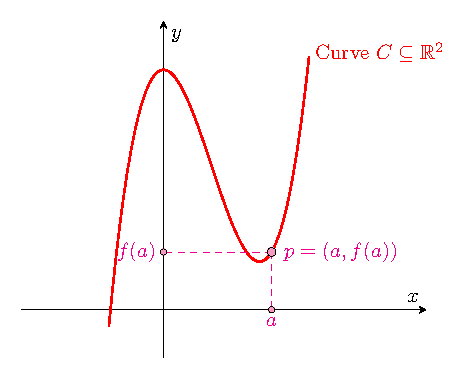
\includegraphics[scale=1]{tangent-space-1.pdf}
%\end{center}
\begin{center}
\begin{minipage}{.49\textwidth}
	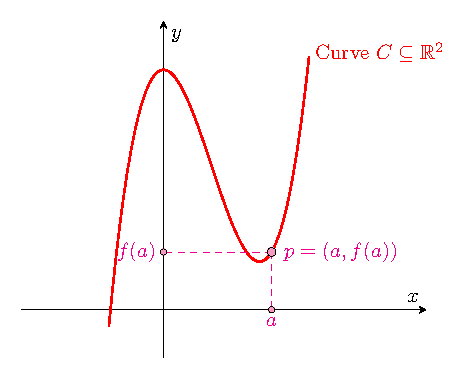
\includegraphics[scale=1]{tangent-space-1.pdf}
\end{minipage}\hfill
\begin{minipage}{.49\textwidth}
	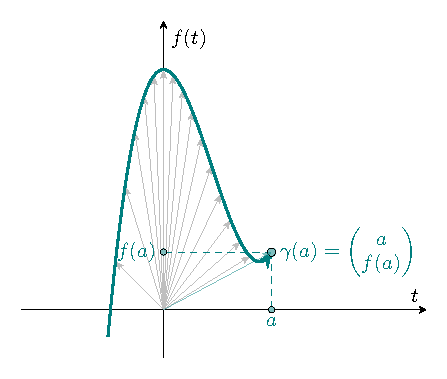
\includegraphics[scale=1]{tangent-space-1-1.pdf}
\end{minipage}
\end{center}
Fix a point $p=(a,f(a))\in C,$ and consider the parametrization \[
\fullfunction{\gamma}{\mathbb{R}}{C\;(\subseteq\R^2)}{t}{
\begin{pmatrix}
	t\\ f(t)
\end{pmatrix}
}.
\]
\newpage
The derivative \(f'(a)
%=\frac{\mathrm{d}f(x)}{\mathrm{d}x}\Big|_{x=a}
\) 
is the slope of the tangent to the curve \(C\) at \(p = (a, f(a))\).
\begin{center}
\begin{minipage}{.49\textwidth}
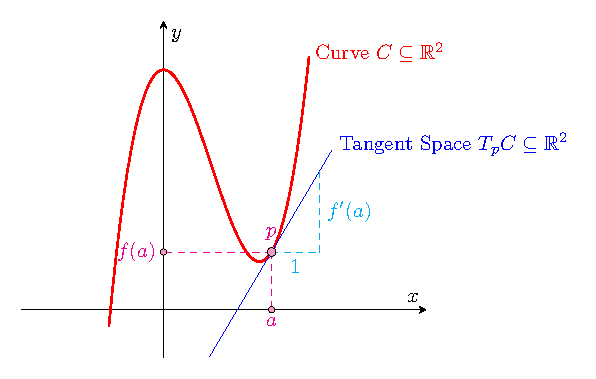
\includegraphics[scale=1]{tangent-space-2.pdf}
\end{minipage}\hfill
\begin{minipage}{.49\textwidth}
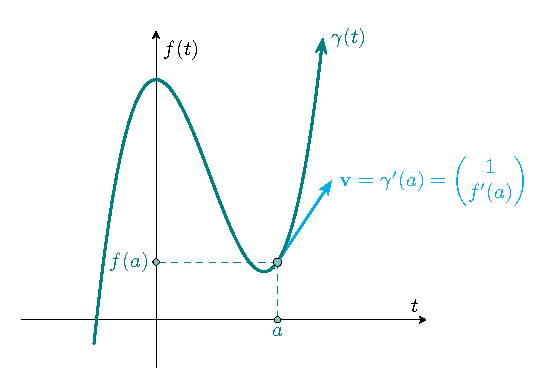
\includegraphics[scale=1]{tangent-space-3-1.pdf}
\end{minipage}
\end{center}
And the velocity of $\gamma$ is \[
\gamma'(t)=\frac{\mathrm{d}\gamma}{\mathrm{d}t}
=\begin{pmatrix}
\frac{\mathrm{d}}{\mathrm{d}t}t\\
\frac{\mathrm{d}}{\mathrm{d}t}f(t)
\end{pmatrix}
=\begin{pmatrix}
1\\ f'(t)\end{pmatrix},
\quad\text{and so}\quad
\gamma'(a)=\begin{pmatrix}
	1\\ f'(a)\end{pmatrix}=\vec{v}\;\in\;T_pC.
\]
%The tangent space to the curve \(C\) at the point \(p \in C\) is the 1-dimensional subspace of \(\mathbb{R}^2\) spanned by the tangent vector \(\vec{v}\), i.e.,
Here, the tangent space $T_pC$ to the curve \(C\) at \(p\) is the set of all scalar multiples of \(\vec v\):
\[
T_pC := \mathrm{span}\set{\vec{v}}=\mathrm{span}\set{\begin{pmatrix} 1 \\ f'(a) \end{pmatrix}}=\set{t\;\begin{pmatrix} 1 \\ f'(a) \end{pmatrix}:t\in\R}
%\mathrm{span}\left\{ \begin{pmatrix} 1 \\ f'(a) \end{pmatrix} \right\} 
\subseteq \mathbb{R}^2.
\]
\begin{center}
	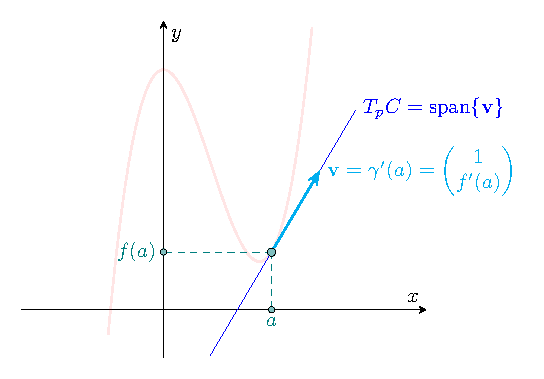
\includegraphics[scale=1]{tangent-space-3-2.pdf}
\end{center}
\newpage
Note that
\begin{itemize}
	\item A \emph{point} $p = (a, f(a)) \in C$ is a \textbf{global location} on the embedded curve $C \subseteq \mathbb{R}^2$; it specifies a particular position in the ambient space.
	\item A \emph{tangent vector} \( \vec{v}=\begin{pmatrix}1\\ f'(a)\end{pmatrix} \in T_pC \subseteq \mathbb{R}^2 \) encodes the curve’s \textbf{local direction and speed} at $p$.
\end{itemize}
%\begin{itemize}
%	\item \emph{Globally}, a point 
%	\[
%	p=(a,f(a))\;\in\;C
%	\;\subseteq\;\R^2
%	\]
%	specifies a \emph{location} on the embedded curve \(C\).
%	\item \emph{Locally}, a tangent vector 
%	\[
%	\vec v
%	=\gamma'(a)
%	=\begin{pmatrix}1\\[3pt]f'(a)\end{pmatrix}
%	\;\in\;T_pC
%	\]
%	encodes the instantaneous \emph{direction} and \emph{speed} of the parametrization at \(p\).
%\end{itemize}
%Note that
%\begin{itemize}
%	\item a \emph{point} \(p=(a,f(a))\in C\) is a \textbf{location} on the curve $C$, and  
%	\item a \emph{tangent vector} \(\vec v\in T_pC\) is an element of \(\mathbb{R}^2\) that encodes ``\textbf{direction+speed}'' at \(p\).  
%\end{itemize}
\begin{center}
\begin{minipage}{.49\textwidth}\centering
	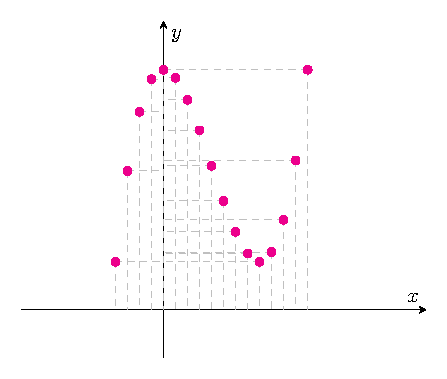
\includegraphics[scale=1]{tangent-space-4-1.pdf}
	Globally, points encode \\\emph{where} we are
\end{minipage}\hfill
\begin{minipage}{.49\textwidth}\centering
	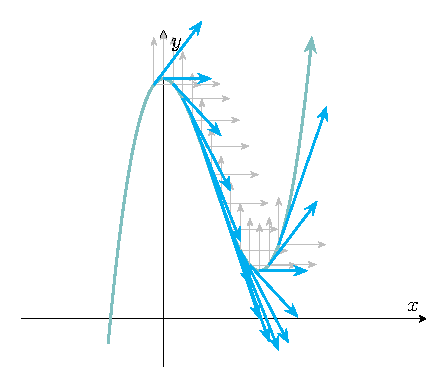
\includegraphics[scale=1]{tangent-space-4-2.pdf}
	Locally, tangent vectors encode\\ \emph{how} we move through that point
\end{minipage}
\end{center}
%Although both live in the same ambient space, points label \emph{where} we are, while vectors label \emph{how} we move through that point.
\newpage\noindent
%\subsection*{Coordinate System on $C$}
We consider the coordinate projections \[
x,y\colon\mathbb{R}^2\to\mathbb{R},
\qquad
x(a,b)=a,
\quad
y(a,b)=b,
\] and restrict them to \(C\subseteq\R^2\). Thus, we obtain two functions: \[
x:C\to\R\quad\text{and}\quad y:C\to\R.
\] 
\begin{center}
\begin{minipage}{.49\textwidth}\centering
	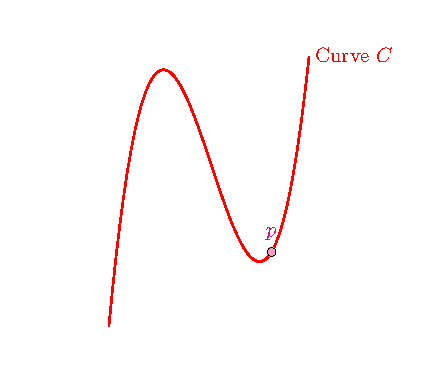
\includegraphics[scale=1]{tangent-space-5-1.pdf}
\end{minipage}\hfill
\begin{minipage}{.49\textwidth}\centering
	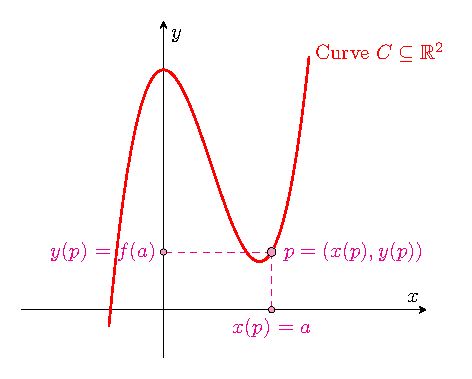
\includegraphics[scale=1]{tangent-space-5-2.pdf}
\end{minipage}
\end{center}
Define a inclusion map \[
\fullfunction{\Phi_C}{C}{\R^2}{p}{(x(p), y(p))}.
\]
%\begin{tikzcd} & \mathbb{R}^2 \arrow[d, "\pi_1", swap] \arrow[dr, "\pi_2"] & \\ C \arrow[ur, "\Phi_C", dashed] \arrow[r, "x|_C", swap] \arrow[rr, "y|_C", bend right] & \mathbb{R} & \mathbb{R} \end{tikzcd}
This map $\Phi_C$\footnote{\color{gray!50}Note that $\Phi_C\in(\R^2)^C, x|_C\in\R^C$ and $y|_C\in\R^C$. Since $\R^2\simeq\R\times\R$ we have $(\R^2)^C\simeq (\R\times\R)^C\simeq\R^C\times\R^C$} records the two ambient coordinates of each point in \(C\subseteq\R^2\).

\newpage\noindent
%\subsection*{Coordinate System on $T_pC$}
We consider the coordinate projections \[
\mathrm{d}x,\mathrm{d}y:T_pC\to\R,\quad \mathrm{d}x(\vec{v})=\mathrm{d}x\left(\begin{pmatrix}
	1& f'(a)
\end{pmatrix}^T\right)=1,\;
\mathrm{d}y(\vec{v})=\mathrm{d}y\left(\begin{pmatrix}
	1& f'(a)
\end{pmatrix}^T\right)=f'(a).
\]
\begin{center}
\begin{minipage}{.49\textwidth}\centering
	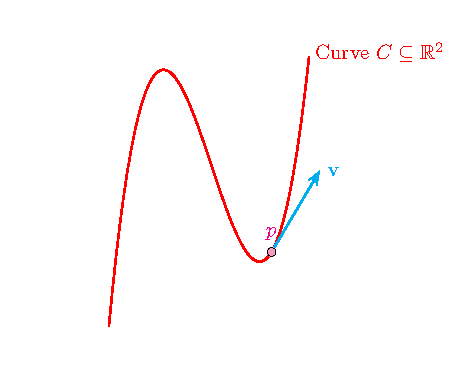
\includegraphics[scale=1]{tangent-space-6-1.pdf}
\end{minipage}\hfill
\begin{minipage}{.49\textwidth}\centering
	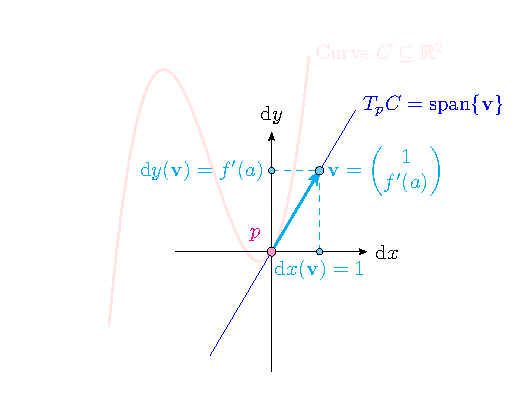
\includegraphics[scale=1]{tangent-space-6-2.pdf}
\end{minipage}
\end{center}
At each \(p=(a,f(a))\in C\), the ambient tangent plane is \[
T_p\R^2
%:=\span\set{\frac{\partial}{\partial x}\Big|_p,\frac{\partial}{\partial y}\Big|_p}=\span\bigl\{\partial_x|_p,\;\partial_y|_p\bigr\}
%:=\span\set{\begin{pmatrix}
%		0\\1
%\end{pmatrix}_{p},\begin{pmatrix}
%1\\ 0
%\end{pmatrix}_{p}}
=\mathrm{span}\{\partial_x\big|_p,\partial_y\big|_p\}
=\set{\alpha\partial_x\big|_p+\beta\partial_y\big|_p:\alpha,\beta\in\R}\;\simeq\;\R^2.
%=\mathrm{span}\{\mathrm{d}x, \mathrm{d}y\}
%=\set{\alpha\mathrm{d}x+\beta\mathrm{d}y:\alpha,\beta\in\R}\;\simeq\;\R^2.
\] 
\begin{center}
	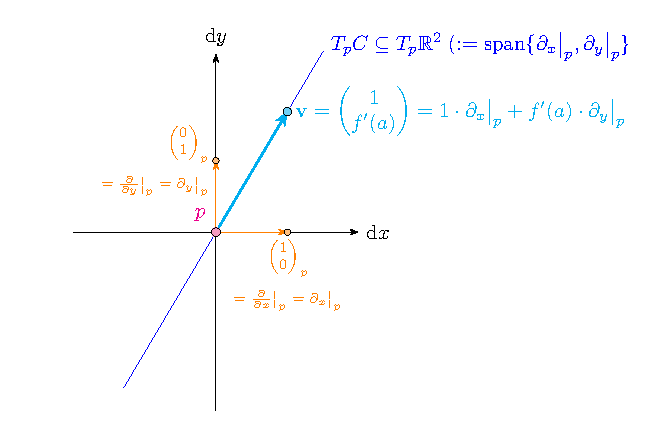
\includegraphics[scale=1]{tangent-space-6-3.pdf}
\end{center}
Define a differential of the inclusion \[
\fullfunction{\Phi_{T_pC}}{T_pC}{\R^2}{\vec{v}}{
\begin{pmatrix}
\mathrm{d}x(\vec{v})& 
\mathrm{d}y(\vec{v})
\end{pmatrix}^T
}
\]
This map \(\Phi_{T_pC}\) records the two components of any tangent vector \(\vec{v}\in T_p\R^2\).

%If the curve is parametrized as $\gamma(t)=(x(t),y(t))$, and $p=\gamma(a)$, then \[
%\vec{v}=\frac{\mathrm{d}}{\mathrm{dt}}\Big|_{t=a}\in T_pC,
%\] and \[
%%d\Phi_{p\in C}=
%\Phi_{T_pC}\left(\vec{v}\right)=\Phi_{T_pC}\left(\frac{\mathrm{d}}{\mathrm{dt}}\Big|_{t=a}\right)
%=\begin{pmatrix}
%	dx/dt\\ dy/dt
%\end{pmatrix}_{t=a}=\begin{pmatrix}
%x'(a)\\ y'(a)
%\end{pmatrix}\in\R^2
%\]

\newpage\noindent
Let
$$
\boxed{
	\omega = dx + f'(a)\,dy \in T_p^*\mathbb{R}^2}
$$ be a \textbf{1-form} defined at point $p = (a, f(a)) \in \mathbb{R}^2$, with the direction $\vec{v}_p = \begin{pmatrix} 1 \\ f'(a) \end{pmatrix}$. 
%This 1-form is a \textit{linear functional}:
In other words, 
\[
\fullfunction{\omega}{T_p\R^2}{\R}{\vec{u} = \begin{pmatrix} u_1 \\ u_2 \end{pmatrix}}{\omega(\vec{u}) = u_1 + f'(a)u_2}
\]
Since $u_1+f'(a)u_2=\begin{pmatrix}
	u_1 & u_2
\end{pmatrix}\begin{pmatrix}
	1\\ f'(a)
\end{pmatrix}=\vec{u}^T\vec{v}_p=\langle\vec{u},\vec{v}_p\rangle$,
$$
\boxed{
	\omega(\vec{u}) = \text{“projection of } \vec{u} \text{ onto } \vec{v}_p = \begin{pmatrix}
		1\\ f'(a)
	\end{pmatrix}\; \text{ direction”}.
}
$$
Let $\vec{proj}_{\vec{v}_p}(\vec{u})=\lambda\vec{v_p}$. Then\[
(\vec{u}-\lambda\vec{v_p})\perp\vec{v_p}\implies\langle\vec{u}-\lambda\vec{v_p},\vec{v}_p\rangle=0\implies\langle\vec{u},\vec{v_p}\rangle-\lambda\langle\vec{v}_p,\vec{v}_p\rangle=0\implies\lambda=\frac{\langle\vec{u},\vec{v}_p\rangle}{\langle\vec{v}_p,\vec{v}_p\rangle}
\] Thus, $\displaystyle\vec{proj}_{\vec{v}_p}(\vec{u})=\frac{\langle\vec{u},\vec{v}_p\rangle}{\langle\vec{v}_p,\vec{v}_p\rangle}\vec{v}_p$:
%
%---
%
%## 🔷 2. Evaluate $\omega(\vec{w})$
%
%Let $\vec{w} = \begin{pmatrix} -1 \\ 2 \end{pmatrix} \in T_p\mathbb{R}^2$. Then:
%
%$$
%\omega(\vec{w}) = dx(\vec{w}) + f'(a)\,dy(\vec{w}) = -1 + 2f'(a).
%$$
%
%This scalar $\omega(\vec{w}) \in \mathbb{R}$ is the **component of $\vec{w}$ along the $\vec{v}_p$** direction.
%
%---
%
%## 🔷 3. Matrix Representation
%
%### 🔹 Vectors as Columns, 1-forms as Rows
%
%* 1-form $\omega = dx + f'(a)\,dy$ is written as a **row vector**:
%
%$$
%\boxed{
%	\omega = \begin{pmatrix} 1 & f'(a) \end{pmatrix}
%}
%$$
%
%* Vector $\vec{w} = (-1,\ 2)^T$ is a **column vector**:
%
%$$
%\boxed{
%	\vec{w} = \begin{pmatrix} -1 \\ 2 \end{pmatrix}
%}
%$$
%
%### 🔹 Evaluation as Dot Product
%
%Then the action is:
%
%$$
%\boxed{
%	\omega(\vec{w}) = \begin{pmatrix} 1 & f'(a) \end{pmatrix} \begin{pmatrix} -1 \\ 2 \end{pmatrix} = -1 + 2f'(a)
%}
%$$
%
%This is a **matrix multiplication** (linear functional applied to a vector):
%
%$$
%\omega(\vec{w}) = \text{(row)} \cdot \text{(column)} = \text{scalar}.
%$$

%---
%
%## 🔷 4. Abstract View
%
%This makes clear:
%
%* $\omega \in T_p^*\mathbb{R}^2$ is a linear functional (1-form),
%* $\vec{w} \in T_p\mathbb{R}^2$ is a direction vector,
%* $\omega(\vec{w})$ measures the component of $\vec{w}$ **in the direction dual to** $\omega$, or equivalently, the **alignment** of $\vec{w}$ with $\vec{v}_p$.
%
%---
%
%## ✅ Final Boxed Summary
%
%**1-form** as function:
%
%$$
%\boxed{
%	\omega : T_p\mathbb{R}^2 \to \mathbb{R},\quad \vec{u} \mapsto \omega(\vec{u}) = u^1 + f'(a)\cdot u^2.
%}
%$$
%
%**Matrix form**:
%
%$$
%\boxed{
%	\omega = \begin{pmatrix} 1 & f'(a) \end{pmatrix}, \quad
%	\vec{w} = \begin{pmatrix} -1 \\ 2 \end{pmatrix}, \quad
%	\omega(\vec{w}) = -1 + 2f'(a).
%}
%$$
%
%This is exactly the **linear algebra realization** of 1-forms acting on tangent vectors.
%
%Would you like to generalize this to arbitrary dimensions or non-Euclidean metrics?

\begin{center}
	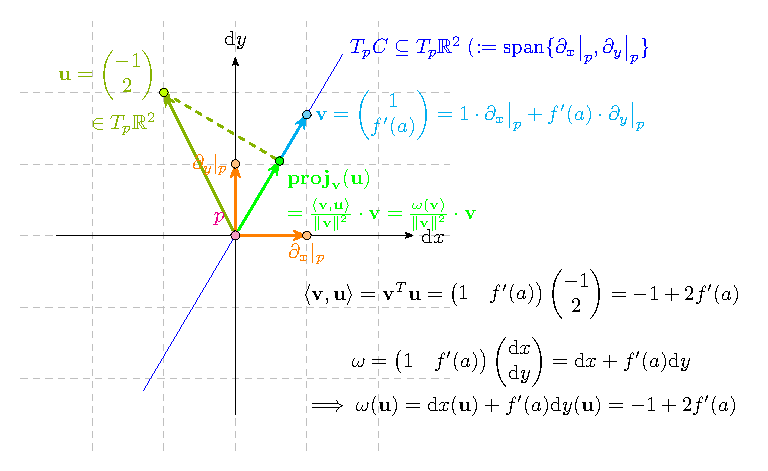
\includegraphics[scale=1.2]{tangent-space-7.pdf}
\end{center}

%Note that \[
%%\vec{v}=\begin{pmatrix}
%%v_1 \\ v_2
%%\end{pmatrix}\mapsto 
%\Phi_{T_pC}(\vec{v})=\begin{pmatrix}
%\mathrm{d}x(\vec{v}) \\ 
%\mathrm{d}y(\vec{v})
%\end{pmatrix}=\begin{pmatrix}
%\begin{pmatrix}1 & 0\end{pmatrix}
%\begin{pmatrix}v_1 \\ v_2\end{pmatrix} \\ \\
%\begin{pmatrix}0 & 1\end{pmatrix}
%\begin{pmatrix}v_1 \\ v_2\end{pmatrix}
%\end{pmatrix}=\begin{pmatrix}
%v_1\\v_2
%\end{pmatrix}.
%\]
%
%\begin{itemize}
%	\item The map \(p\mapsto(x(p),y(p))\) simply records the two ambient coordinates
%	of each point in \(C\subset\R^2\).
%	\item The map \(v\mapsto(dx(v),dy(v))\) records the two components of any tangent
%	vector \(v\in T_p\R^2\).
%	\item The 1-form \(\alpha=\hat w_1\,dx+\hat w_2\,dy\) is precisely the functional
%	that takes each tangent vector and returns its scalar component in the fixed
%	direction \(\hat w\).
%\end{itemize}
%
%\subsection*{Definition of a \(1\)\,-form on \(\R^2\)}
%
%Let \(U\subseteq\R^2\) be open.  In the standard coordinates \((x,y)\) one has the coordinate vector fields
%\[
%\partial_x\big|_p \;=\;\frac{d}{dt}\Bigl(x+p_x,y\Bigr)\Bigl|_{t=0},
%\quad
%\partial_y\big|_p \;=\;\frac{d}{dt}\Bigl(x,y+p_y\Bigr)\Bigl|_{t=0},
%\]
%and hence
%\[
%T_p\R^2 \;=\;\mathrm{span}\bigl\{\partial_x\big|_p,\;\partial_y\big|_p\bigr\}\;\cong\;\R^2.
%\]
%Its dual space is
%\[
%T_p^*\R^2
%\;=\;
%\mathrm{Hom}_\R\bigl(T_p\R^2,\;\R\bigr)
%\;=\;
%\mathrm{span}\bigl\{\,dx\big|_p,\;dy\big|_p\bigr\},
%\]
%where \(dx\big|_p,dy\big|_p\) satisfy
%\[
%dx\big|_p\bigl(\partial_x\big|_p\bigr)=1,\quad dx\big|_p\bigl(\partial_y\big|_p\bigr)=0,
%\quad
%dy\big|_p\bigl(\partial_x\big|_p\bigr)=0,\quad dy\big|_p\bigl(\partial_y\big|_p\bigr)=1.
%\]
%\begin{definition}
%	A \emph{\(1\)\,-form} on \(U\) is a smooth section of the cotangent bundle:
%	\[
%	\omega
%	\;:\;
%	p\;\longmapsto\;\omega_p
%	\;\in\;
%	T_p^*\R^2,
%	\]
%	i.e.\ \(\omega\in\Gamma\bigl(T^*U\bigr)\).  Equivalently,
%	\[
%	\omega_p\;=\;A(p)\,dx\big|_p\;+\;B(p)\,dy\big|_p,
%	\]
%	for some \(A,B\in C^\infty(U)\).
%\end{definition}

\newpage
\subsection*{Example $C:y=x^2$}
We take \[
C=\bigl\{(x,y)\in\R^2\mid y=x^2\bigr\}.
\]
\begin{center}
\begin{minipage}{.49\textwidth}
	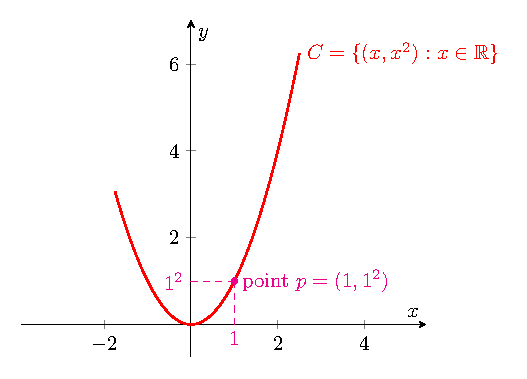
\includegraphics[scale=1]{tangent-space-example-1.pdf}
\end{minipage}
\begin{minipage}{.49\textwidth}
	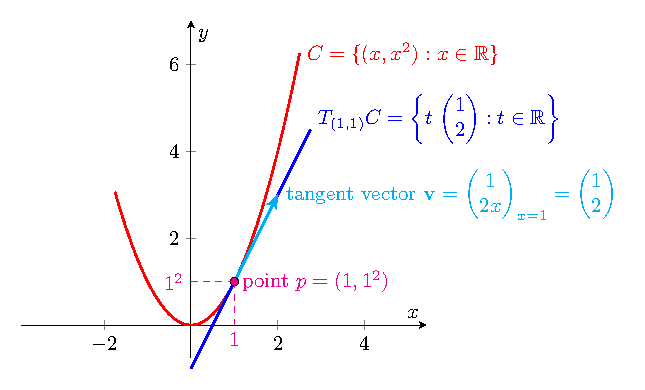
\includegraphics[scale=1]{tangent-space-example-2.pdf}
\end{minipage}
\end{center}
Set \(a=1\).  Then the point \(p=(1,1)\) lies on \(C\). 
\begin{center}
	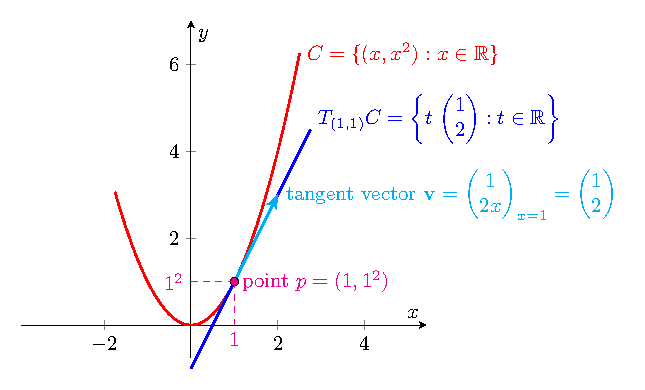
\includegraphics[scale=1]{tangent-space-example-2.pdf}
\end{center}
Since \(f'(x)=2x\), we have
\[
\vec v=\begin{pmatrix}1\\f'(1)\end{pmatrix}=\begin{pmatrix}1\\2\end{pmatrix}.
\] Thus
\[
T_pC
=\mathrm{span}\set{\begin{pmatrix}
1\\ 2
\end{pmatrix}}=\set{t\,\begin{pmatrix}1\\ 2\end{pmatrix}\;:\;t\in\mathbb{R}}
\subseteq\mathbb{R}^2.
\]
\newpage\noindent
%Define the global parametrization \[
%\fullfunction{\gamma}{\mathbb{R}}{C\;(\subseteq\R^2)}{t}{\bigl(t,f(t)\bigr)}.
%\] 
%Its inverse is \[
%\fullfunction{\gamma^{-1}}{C\;(\subseteq\R^2)}{\R}{(x,y)}{x}.
%\] Thus every \(p\in C\) is uniquely represented by \(p=\gamma(t)\).
Consider a inclusion map \[
\fullfunction{\Phi_C}{C}{\R^2}{p}{(x(p), y(p))}.
\]
\begin{center}
\begin{minipage}{.45\textwidth}
	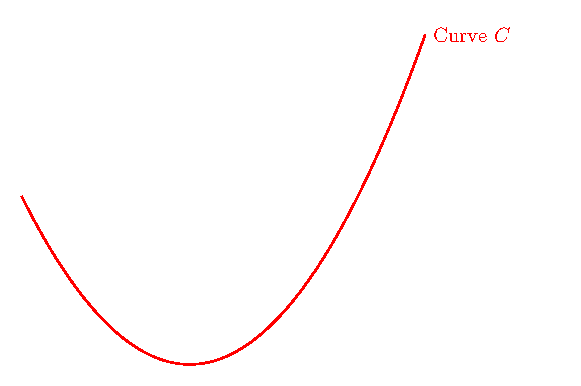
\includegraphics[scale=1]{tangent-space-example-3.pdf}
\end{minipage}
\begin{minipage}{.45\textwidth}
	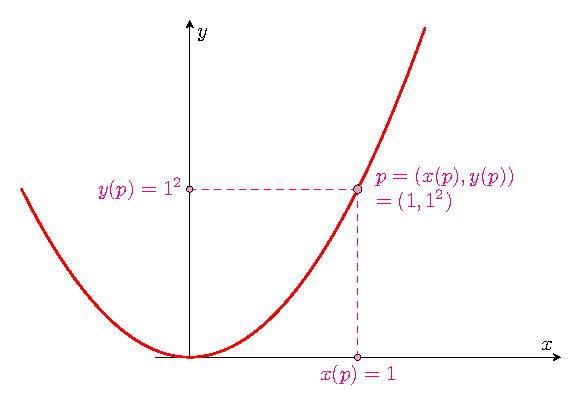
\includegraphics[scale=1]{tangent-space-example-3-1.pdf}
\end{minipage}
\end{center}
Then a differential of the inclusion map is \[
\fullfunction{\Phi_{T_pC}}{T_pC}{\R^2}{\vec{v}}{
	\begin{pmatrix}
		\mathrm{d}x(\vec{v})\\
		\mathrm{d}y(\vec{v})
	\end{pmatrix}
}
\]
\begin{center}
\begin{minipage}{.49\textwidth}
	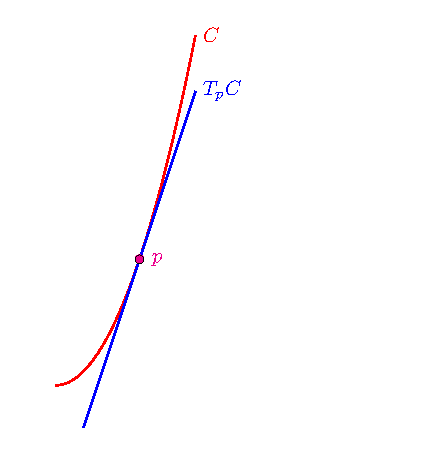
\includegraphics[scale=1]{tangent-space-example-4-1.pdf}
\end{minipage}\hfill
\begin{minipage}{.49\textwidth}
	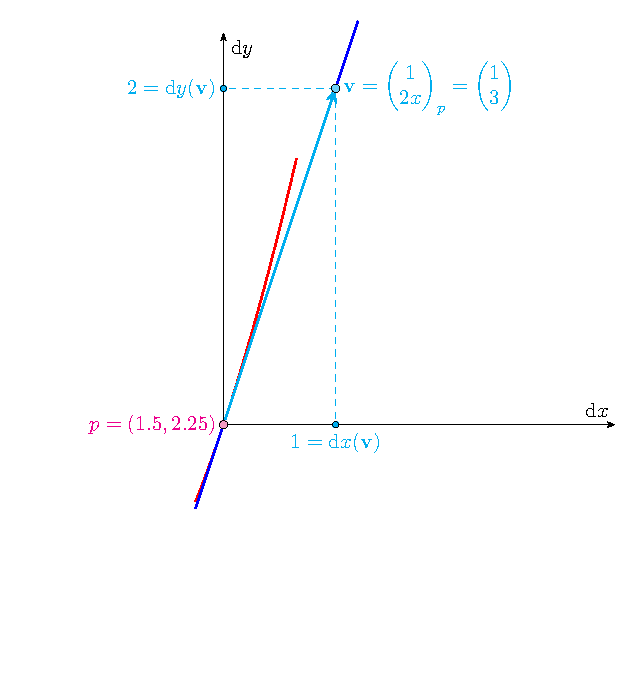
\includegraphics[scale=.8]{tangent-space-example-4.pdf}
\end{minipage}
\end{center}

\newpage\noindent
%\section*{The 1-Form \(\omega\)}
Consider the differential 1-form on \(\mathbb{R}^2 \setminus \{0\}\):
\[
\omega = \frac{-y}{x^2 + y^2} \, dx + \frac{x}{x^2 + y^2} \, dy.
\]
This 1-form corresponds to the angular differential \(d\theta\) in polar coordinates. 

%It satisfies:
%\[
%\omega = d\theta \quad \text{(locally on } \mathbb{R}^2 \setminus \{0\} \text{)}.
%\]

%\section*{Integral on the Unit Circle}

Let \( C \subseteq \mathbb{R}^2 \) be the unit circle centered at the origin, parametrized by:
\[
\gamma(\theta) = \begin{pmatrix}
\cos\theta\\ \sin\theta
\end{pmatrix}, \quad \theta \in [0, 2\pi],
\]
with counterclockwise orientation.
\begin{center}
	\begin{minipage}{.49\textwidth}\centering
		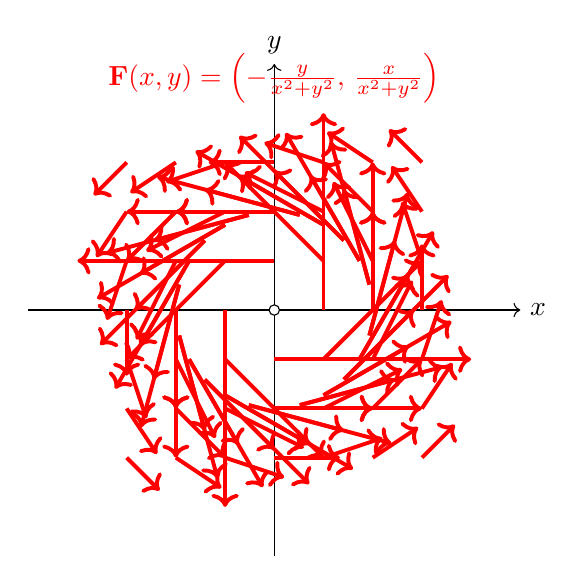
\begin{tikzpicture}[scale=1.25]
			%	\draw[dashed, gray!20] (-4,-4) grid (4,4);
			% Axes
			\draw[->] (-2.5,0) -- (2.5,0) node[right] {$x$};
			\draw[->] (0,-2.5) -- (0,2.5) node[above] {$y$};
			% Desired arrow length
			\def\arrowlen{1}	
			% Loop over integer grid points
			\foreach \X in {-1.5,-1,-.5,0,.5,1,1.5} {
				\foreach \Y in {-1.5,-1,-.5,0,.5,1,1.5} {
					% Compute radius r = sqrt(x^2+y^2)
					\pgfmathsetmacro{\r}{\X*\X + \Y*\Y}
					
					\ifdim \r pt=0pt
					% At (0,0): singularity
					\fill[white,draw=black] (0,0) circle (1.5pt);
					\else
					% Compute unit‐tangent components then scale
					\pgfmathsetmacro{\dx}{(-\Y/\r)*\arrowlen}
					\pgfmathsetmacro{\dy}{(\X/\r)*\arrowlen}
					
					% Draw the arrow
					\draw[->, line width=.5mm, red]
					(\X,\Y) -- ++(\dx,\dy);
					\fi
				}
			}
			\foreach \t in {0,15,...,345}{
				\pgfmathsetmacro\x{cos(\t)}
				\pgfmathsetmacro\y{sin(\t)}
				% On r=1, F = (-y,x)
				\pgfmathsetmacro\dx{(-\y)*\arrowlen}
				\pgfmathsetmacro\dy{(\x)*\arrowlen}
				\draw[->, line width=.5mm, red] 
				(\x,\y) -- ++(\dx,\dy);
			}
			\def\arrowlen{1.5}
			\foreach \t in {0,15,...,345}{
				\pgfmathsetmacro\x{cos(\t)}
				\pgfmathsetmacro\y{sin(\t)}
				% On r=1, F = (-y,x)
				\pgfmathsetmacro\dx{(-\y)*\arrowlen}
				\pgfmathsetmacro\dy{(\x)*\arrowlen}
				\draw[->, line width=.5mm, red] 
				(\x,\y) -- ++(\dx,\dy);
			}
			
			%--- Annotations -----------------------------------------
			\node[above, red] at (0,2)
			{$\vec{F}(x,y)=\left(-\tfrac{y}{x^2+y^2},\,\tfrac{x}{x^2+y^2}\right)$};
		\end{tikzpicture}
	\end{minipage}
	\begin{minipage}{.49\textwidth}\centering
		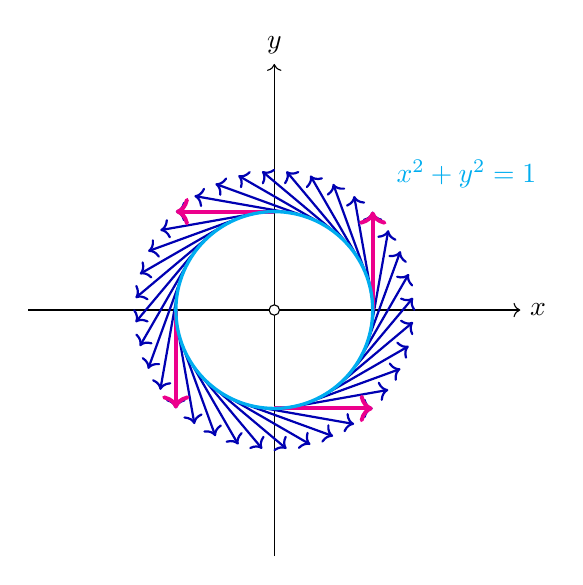
\begin{tikzpicture}[scale=1.25]
			%	\draw[dashed, gray!20] (-4,-4) grid (4,4);
			% Axes
			\draw[->] (-2.5,0) -- (2.5,0) node[right] {$x$};
			\draw[->] (0,-2.5) -- (0,2.5) node[above] {$y$};
			\fill[white,draw=black] (0,0) circle (1.5pt);
			\def\arrowlen{1}
			\foreach \t in {0,10,...,350}{
				\pgfmathsetmacro\x{cos(\t)}
				\pgfmathsetmacro\y{sin(\t)}
				% On r=1, F = (-y,x)
				\pgfmathsetmacro\dx{(-\y)*\arrowlen}
				\pgfmathsetmacro\dy{(\x)*\arrowlen}
				\draw[->, thick, blue!70!black] 
				(\x,\y) -- ++(\dx,\dy);
			}
			\foreach \t in {0,90,180,270}{
				\pgfmathsetmacro\x{cos(\t)}
				\pgfmathsetmacro\y{sin(\t)}
				% On r=1, F = (-y,x)
				\pgfmathsetmacro\dx{(-\y)*\arrowlen}
				\pgfmathsetmacro\dy{(\x)*\arrowlen}
				\draw[->, line width=.5mm, magenta] 
				(\x,\y) -- ++(\dx,\dy);
			}
			%--- Draw contour C with orientation --------------------
			\draw[cyan, very thick]
			(0,0) circle (1)
			node[above right=2cm] {$x^2+y^2=1$};
		\end{tikzpicture}
	\end{minipage}
\end{center}
TBA...

%We compute the line integral:
%\[
%\int_C \omega = \int_0^{2\pi} \left[ \frac{-\sin\theta}{1} \cdot (-\sin\theta) + \frac{\cos\theta}{1} \cdot \cos\theta \right] d\theta
%= \int_0^{2\pi} ( \sin^2\theta + \cos^2\theta ) d\theta = \int_0^{2\pi} 1 \, d\theta = 2\pi.
%\]

%\section*{Geometric Visualization}
%\begin{center}
%	\begin{tikzpicture}[scale=3, >=Latex]
%		
%		% Axes
%		\draw[->] (-1.2,0) -- (1.4,0) node[right] {\(x\)};
%		\draw[->] (0,-1.2) -- (0,1.4) node[above] {\(y\)};
%		
%		% Unit circle
%		\draw[thick, blue] (0,0) circle (1);
%		\node at (1.2,0.2) {\(C: x^2 + y^2 = 1\)};
%		
%		% Orientation arrow on circle
%		\draw[->, thick, blue] (0.707,0.707) arc (45:135:1cm);
%		\node at (-0.4,1.05) {Counterclockwise};
%		
%		% Sample points with angular field vector
%		\foreach \angle in {30, 60, 120, 150, 210, 240, 300, 330} {
%			\coordinate (P) at ({cos(\angle)}, {sin(\angle)});
%			\coordinate (V) at ({-sin(\angle)*0.15}, {cos(\angle)*0.15});
%			\draw[->, thick, red] (P) -- ($(P)+(V)$);
%		}
%		
%		% Origin
%		\filldraw (0,0) circle (0.3pt) node[below left] {\(0\)};
%		
%		% Label for 1-form
%		\node at (0,-1.05) {\(\omega = \dfrac{-y}{x^2 + y^2}dx + \dfrac{x}{x^2 + y^2}dy\)};
%		
%	\end{tikzpicture}
%\end{center}

%\section*{Conclusion}

%The integral of \( \omega \) over the unit circle oriented counterclockwise is:
%\[
%\boxed{ \oint_C \omega = 2\pi }
%\]
%
%This form is closed (since \( d\omega = 0 \)) but not exact globally on \( \mathbb{R}^2 \setminus \{0\} \) because the domain is not simply connected. This corresponds to the non-vanishing of the first de Rham cohomology group \( H^1(\mathbb{R}^2 \setminus \{0\}) \cong \mathbb{R} \), and this integral represents the generator.


\newpage
\begin{table}\centering
\begin{tabularx}{\textwidth}{p{3cm}|p{5cm}|X}
	\toprule[1.2pt]
	\textbf{Degree} $k$ & \textbf{Object} & \textbf{Vector Space} \\ \midrule
	0-form & Scalar function & $f(p)\in\R$ \\
	1-form & Linear Functional & $(T_p\R^n\to\R)\in T_p^*\R^n$\\
	2-form & TBA & TBA\\
	TBA & & \\
	\bottomrule[1.2pt]
\end{tabularx}
\end{table}

\end{document}
